\documentclass[12pt,a4paper]{article}

%% Packages
\usepackage[utf8]{inputenc}
\usepackage[T1]{fontenc}
\usepackage{lmodern}
\usepackage{graphicx}
\usepackage{amsmath,amssymb}
\usepackage{booktabs}
\usepackage{natbib}
\usepackage{geometry}

\usepackage{caption} % For caption spacing
\usepackage{subcaption} % For sub-figures
\usepackage{graphicx}
\usepackage{float}

\geometry{margin=2.5cm}

%% Title and Author
\title{Residential Segregation in Brazil: An Inference Framework Based study for Selected Cities}

\author{
Renan Xavier Cortes\\
Department of Statistics\\
Federal university of Rio Grande do Sul\\
Porto Alegre, Brazil\\
\texttt{renan.cortes@ufrgs.br}
\and
Second Author\\
Department Name\\
University Name\\
City, Country
}

\date{\today}

\usepackage{Sweave}
\begin{document}
\Sconcordance{concordance:draft_v4.tex:draft_v4.Rnw:1 37 1 1 0 137 1}


\maketitle

\begin{abstract}
This is a simple abstract. It briefly explains the objective,
methods, main results, and conclusions of the study.
\end{abstract}

\noindent\textbf{Keywords:} Keyword1; Keyword2; Keyword3

\section{Introduction}\label{sec:introduction}

Residential segregation is a major topic of study

\cite{massey1988dimensions} goes here \cite{allen2015more}

Talk about it is census tract level (and not neighborhood)


\section{Related work}\label{sec:related-work}

\cite{cortes2020open}

Here, in this section I cite renan, \cite{rey2021comparative}

I also cite all brazilian papers of the literature
\cite{sousa2023nacional}
\cite{deSousaFilho2022nationwide}
\cite{barber2018cardioelsa}
\cite{barros2018unevengeographies}
\cite{barros2024saopaulolondres}
\cite{strauch2026bh20102022}
\cite{danilofranca2022fortaleza}

Why we chose those cities

\section{Framework} \label{subsec:statistical-summaries}

Here, I discuss the hyphotesis present the null hyphothesis and alternative hypothesis

and limitaitons of the approach recovering the Reviewer comments.

Discuss the dimensions o Massey...

Queen matrix

Segreagation measures choses

\section{Results}\label{subsec:statistical-summaries}

Hardware, 

\subsection{Point Estimation of segregation measures}\label{sec:sampling}


Here I put the maps
Here I put all point measurements and discuss



\begin{figure}[htbp]
    \centering
    
    \begin{subfigure}{0.48\textwidth}
        \centering
        \includegraphics[width=\linewidth]{figures/seg_profile_4314902.png}
        \caption{Porto Alegre, RS}
        \label{fig:1}
    \end{subfigure}
    \hfill
    \begin{subfigure}{0.48\textwidth}
        \centering
        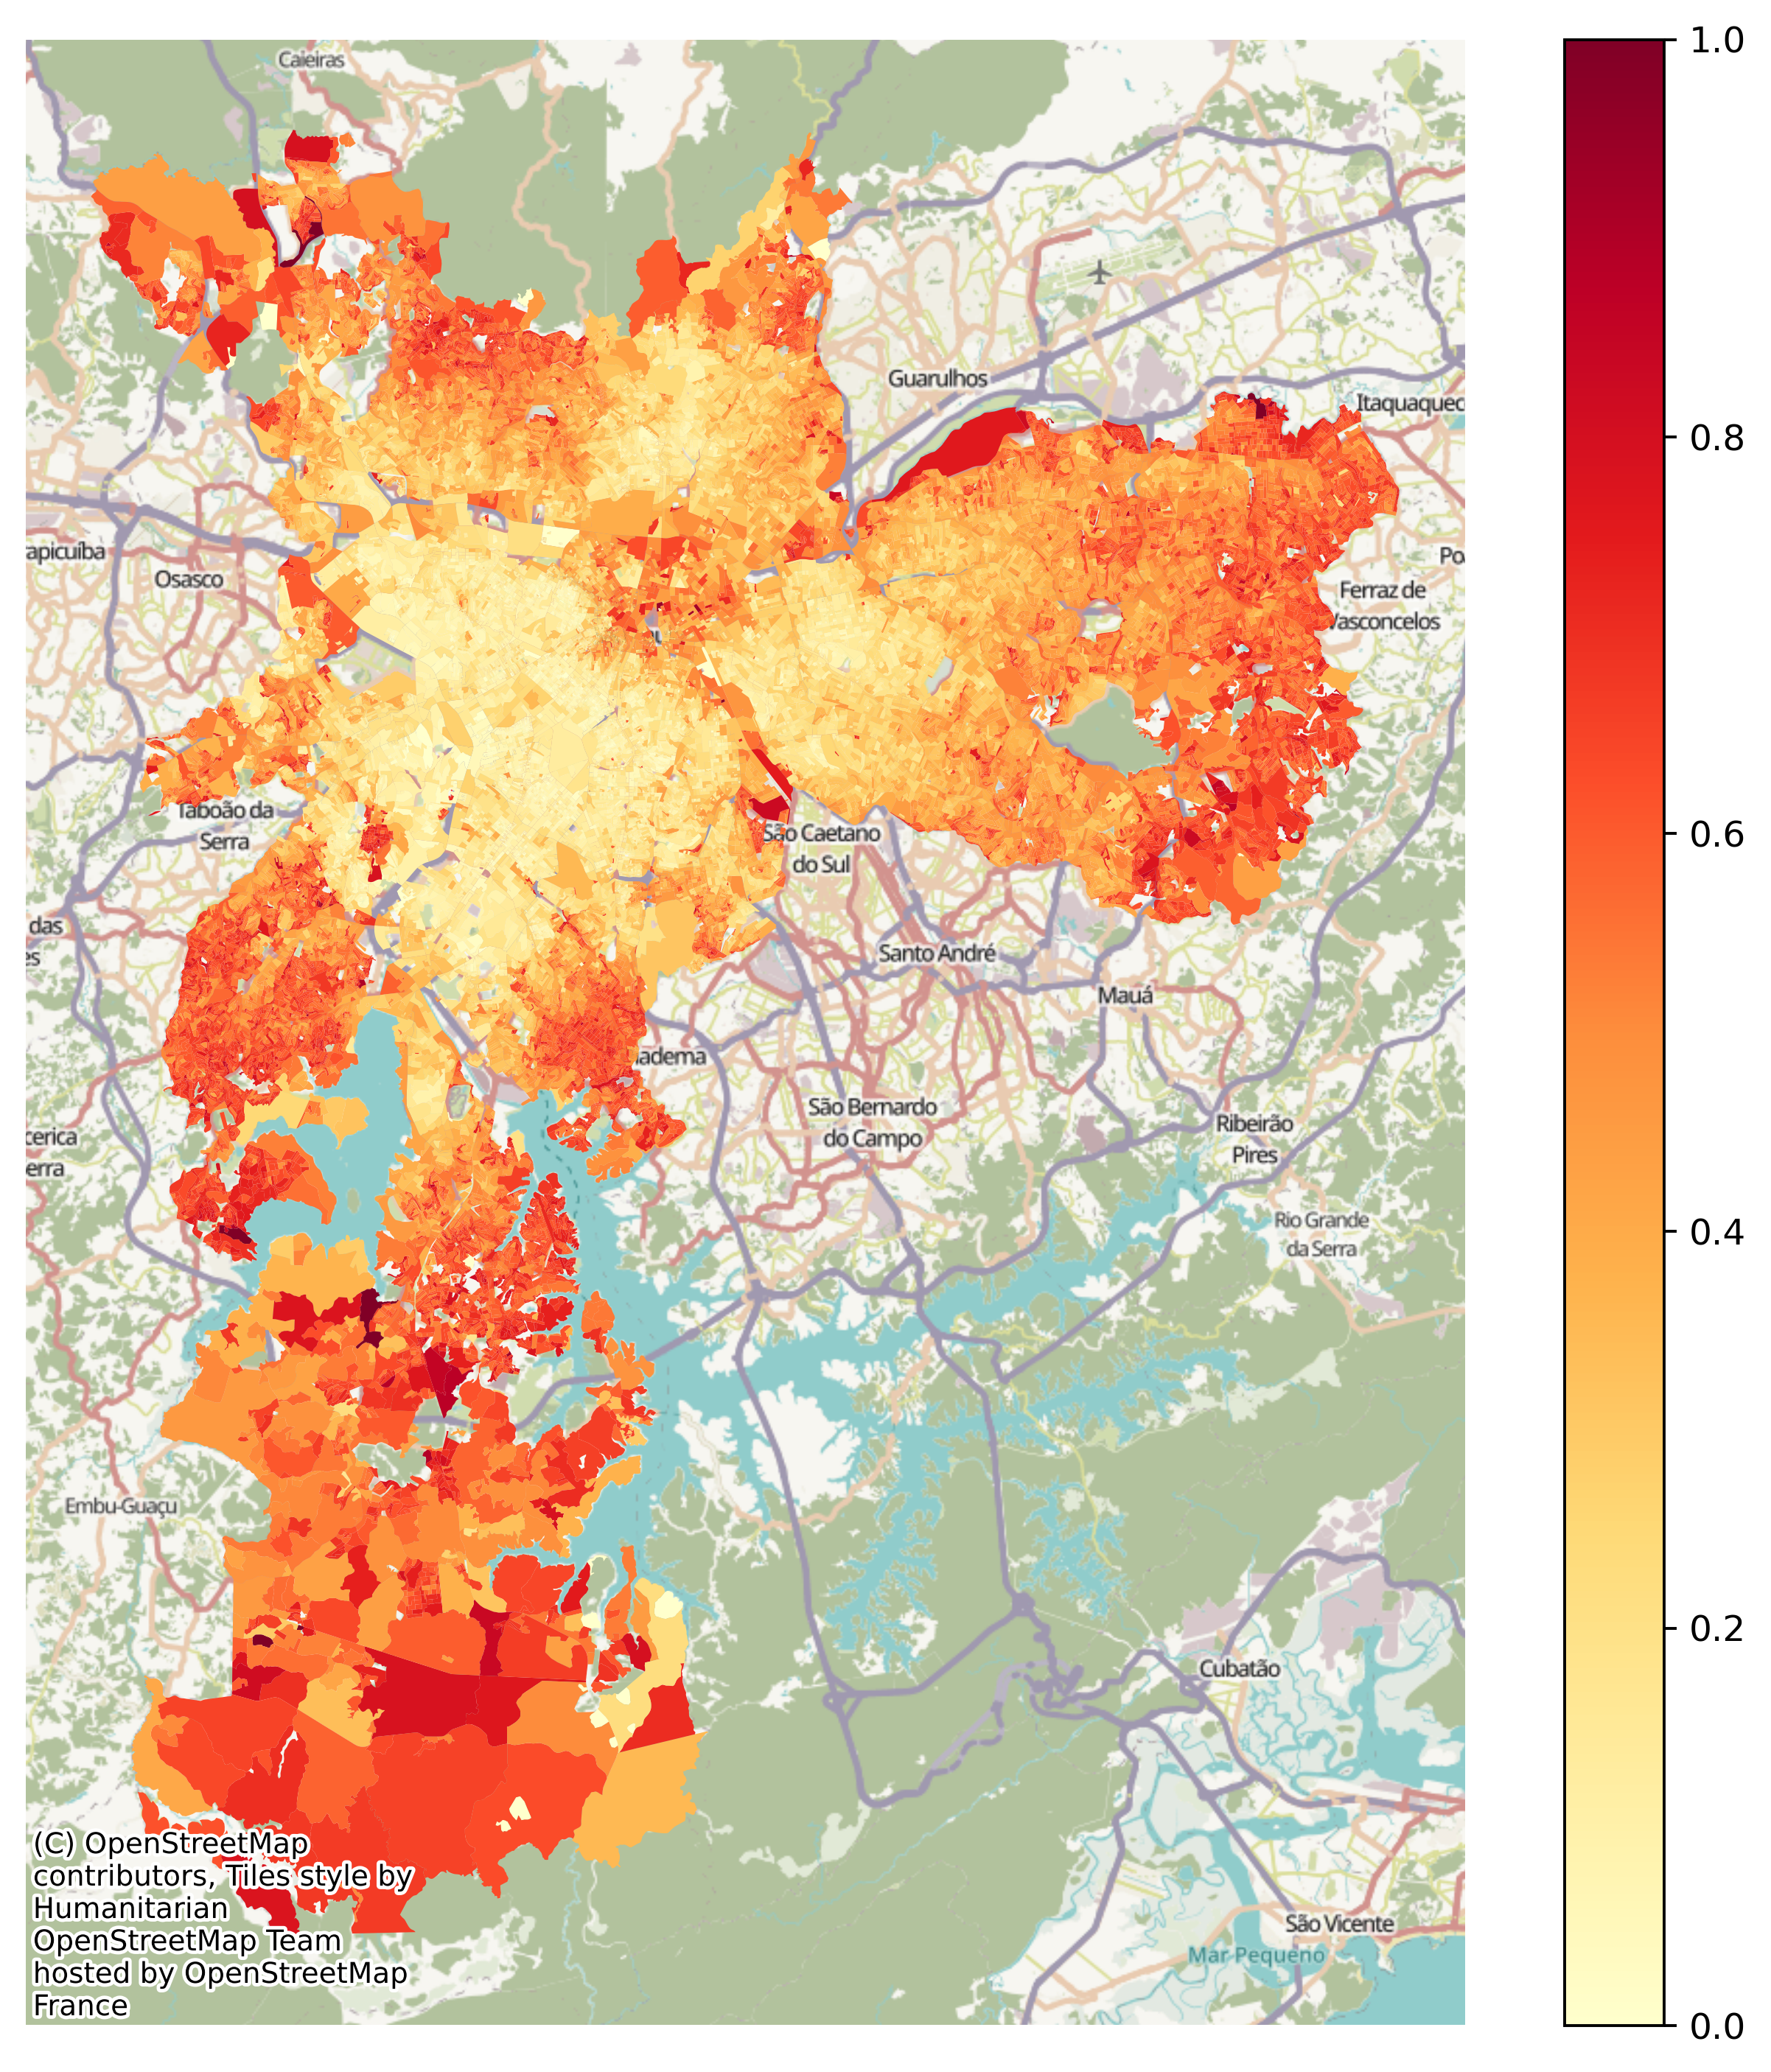
\includegraphics[width=\linewidth]{figures/seg_profile_3550308.png}
        \caption{São Paulo, SP}
        \label{fig:2}
    \end{subfigure}
    
    \vspace{0.5cm}
    
    \begin{subfigure}{0.48\textwidth}
        \centering
        \includegraphics[width=\linewidth]{figures/seg_profile_3304557.png}
        \caption{Rio de Janeiro, RJ}
        \label{fig:3}
    \end{subfigure}
    \hfill
    \begin{subfigure}{0.48\textwidth}
        \centering
        \includegraphics[width=\linewidth]{figures/seg_profile_3106200.png}
        \caption{Belo Horizonte, MG}
        \label{fig:4}
    \end{subfigure}
    
    \caption{Composition of all selected cities}
    \label{fig:2x2grid}
\end{figure}

\subsection{Inference results}\label{sec:sampling}

Computational challenges

\begin{figure}[H]
    \centering
    \includegraphics[width=0.99\textwidth]{figures/grid_plot_4314902_systematic.png}
    \caption{Point Estimation with systematic approach}
    \label{fig:grid_plot_4314902_systematic}
\end{figure}

\begin{figure}[H]
    \centering
    \includegraphics[width=0.99\textwidth]{figures/grid_plot_4314902_evenness.png}
    \caption{Point Estimation with evenness approach}
    \label{fig:grid_plot_4314902_evenness}
\end{figure}

\begin{figure}[H]
    \centering
    \includegraphics[width=0.99\textwidth]{figures/grid_plot_4314902_geographic_permutation.png}
    \caption{Point Estimation with Geographic Permutation approach}
    \label{fig:grid_plot_4314902_geographic_permutation}
\end{figure}


\section{Discussion and Future Work}\label{sec:statistical-summaries}


More cities
Comparative framework detangling with shapley
Street network based.

%% Bibliography
\bibliographystyle{plainnat}
\bibliography{references}

\end{document}

